\chapter{Описание механизма построения запросов PostgreSQL}

\section{План запроса}

SQL - декларативный язык: запрос определяет, какие данные необходимо получить, но не указывает, как именно их получить. Запрос может быть выполнен несколькими способами. Планировщик запросов перебирает все эти способы и выбирает наиболее быстрый и экономичный по ресурсам. План выполнения представляется в виде дерева, которое можно вывести с помощью команды EXPLAIN. 

\begin{lstlisting}[language=SQL, caption={План выполнения с помощью EXPLAIN запроса "SELECT COUNT(x) FROM a UNION ALL SELECT SUM(x) FROM b"}, label={lst:explain_plan}]
Append  (cost=41.88..83.78 rows=2 width=8)
   ->  Aggregate  (cost=41.88..41.88 rows=1 width=8)
         ->  Seq Scan on a  (cost=0.00..35.50 rows=2550 width=4)
   ->  Aggregate  (cost=41.88..41.88 rows=1 width=8)
         ->  Seq Scan on b  (cost=0.00..35.50 rows=2550 width=4)
\end{lstlisting}

\begin{figure}[htbp]
	\centering
	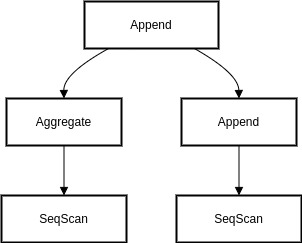
\includegraphics[width=0.33\textwidth]{graphics/query_tree.jpg}
	\caption{Дерево запроса "SELECT COUNT(x) FROM a UNION ALL SELECT SUM(x) FROM b"}
	\label{fig:query_tree}
\end{figure}

Все запросы можно разделить на группы по типам планов выполнения, то есть по видам запросов в зависимости от их плана. Определяющим фактором в данном случае является наличие определённых узлов в дереве плана. Например, запрос на Рис. 2.1 можно отнести к типам Append, Aggregate и Seq Scan. Запросы с множественными типами узлов затрудняют выявление того узла, который вызывает ухудшение производительности запроса. Поэтому желательно генерировать такие запросы, которые можно отнести только к одному типу узла. Однако это не всегда возможно — если запрос должен прочитать таблицу, то будет включён узел, связанный с чтением таблицы. Выполнение операций JOIN также требует чтения таблиц. Тем не менее, при работе с JOIN-операциями можно избежать использования агрегатных функций, операций сортировки и других операций. Это позволяет свести количество различных узлов в дереве плана к минимуму.

Цель состоит в генерации запросов, которые обеспечат присутствие заданного узла в плане выполнения. Для этого можно использовать две стратегии.

Первая стратегия основана на добавлении в запрос ключевых слов, гарантирующих включение определённых узлов. Например, если требуется узел типа Aggregate, в запрос можно добавить ключевые слова для выполнения агрегатных функций, таких как COUNT(), MAX() и т.д. Если нужен узел Append, то запрос должен содержать оператор UNION ALL для объединения результатов нескольких запросов. Однако для получения узла Seq Scan это не всегда применимо. Существует несколько способов чтения таблицы, и наиболее подходящий выбирается в зависимости от условий. В PostgreSQL для этой цели используется стоимостной оптимизатор, который оценивает потенциальные планы выполнения по ресурсоемкости (включая операции ввода-вывода и загрузку процессора). Каждый план получает числовую оценку стоимости, и план с наименьшей стоимостью выбирается оптимизатором для выполнения запроса.

Вторая стратегия заключается в анализе стоимости для всех узлов, выполняющих схожие задачи, и формировании таких условий в запросе, которые заставят оптимизатор выбрать требуемый узел.

\section{Анализ узлов дерева запросов.}

\subsection{Узлы для сканирования}

\subsubsection{Последовательное сканирование}

Последовательное сканирование - это один из типов узлов отвечающих за чтение таблицы и является самым эффективным способом прочитать всю таблицу или её значительную часть. Это особенно полезно при низкой селективности запроса. Напротив, при высокой селективности, когда требуется извлечь лишь небольшую часть строк из таблицы, лучше использовать индекс.

Стоимость последовательное сканирования не зависит от селективности. Пусть у нас есть условный оператор WHERE в запросе и N $-$ количество условий в запросе.
\begin{equation}
\begin{array}{c}
SeqScanCost =  seqPageCost \, *  \,  relpages  \,  + \,  cpuTupleCost  \,  *  \, \\
* \, reltuples  \,  +  \, cpuOperatorCost  \, * \,  N  \, * \,  reltuples
\label{seq_scan_cost}
\end{array}
\end{equation}

\begin{itemize}
    \item $seqPageCost$ $-$ стоимость последовательного сканирования 1 страницы;
    \item $relpages$ $-$ количество страниц;
    \item $cpuTupleCost$ $-$ стоимость обработки одной версии строк;
    \item $reltuples$ $-$ количество версий строк;
    \item $cpuOperatorCost$ $-$ стоимость условной операции
\end{itemize}

\subsubsection{Индексное сканирование}

Оценка производительности индексного сканирования включает в себя два компонента: оценку затрат на доступ к индексу и оценку затрат на чтение страниц таблицы. Очевидно, что индексная часть этой оценки зависит от конкретного метода доступа. Для B-деревьев основные затраты связаны с чтением индексных страниц и обработкой строк на этих страницах. В данной работе рассматривается исключительно индексирование с использованием B-дерева. Для определения количества прочитанных страниц и строк необходимо учитывать общий объем данных и селективность условий. Доступ к индексным страницам может быть случайным, поскольку страницы, которые логически соседствуют, могут физически располагаться в разных местах на диске. Важно отметить, что оценка ввода-вывода зависит также от того, насколько хорошо физическое расположение строк на диске соответствует порядку их извлечения с помощью выбранного метода доступа.

\textbf{Хорошая корреляция.} Если физический порядок версий на диске идеально коррелирует с логическим порядком идентификаторов в индексе, то, читая версии строк одну за другой, узел Index Scan будет последовательно переходить от страницы к странице и обратится к каждой из них только один раз. Формула для подсчёта индексного сканирования в этом случае:
\begin{equation}
    IndexScanCost = idxCost +tblCost
\end{equation}
\begin{equation}
    \begin{array}{c}
        idxCost = randomPageCost * relpages * sel + cpuIndexTupleCost * reltuples * sel \, + \\
        + \, cpuOperatorCost * reltuples * sel
    \end{array}
\end{equation}
\begin{equation}
    \begin{array}{c}
         tblCost = seqPageCost * relpages * sel + cpuTupleCost * reltuples * sel + \\ 
         + \, cpuOperatorCost * reltuples * sel
    \end{array}
\end{equation}

\begin{itemize}
    \item $idxCost$ $-$ стоимость доступа к индексу;
    \item $tblCost$ $-$ стоимость чтения табличных страниц;
    \item $randomPageCost$ $-$ стоимость случайного сканирования 1 страницы;
    \item $relpages, \ reltuples$ $-$ страницы и версии строк индекса таблицы для $idxCost$ и страницы и версии строк самой таблицы для $tblCost$;
    \item $cpuIndexTupleCost$ $-$ стоимость обработки одной индексной версии строк;
    \item $sel$ $-$ селективность.
\end{itemize}

\textbf{Плохая корреляция.} Чем ниже корреляция, тем выше вероятность того, что следующая версия строки, идентификатор которой возвращает метод доступа, окажется на другой странице. В результате узел Index Scan вместо последовательного чтения страниц «перескакивает» с одной страницы на другую, и в предельном случае количество обращений к страницам может равняться числу выбираемых строк. Однако было бы некорректным просто заменить параметр $seqPageCost$ на $randomPageCost$, а $relpages$ на $reltuples$ в приведенной формуле. Стоимость, которую мы видим в плане выполнения, как правило, значительно ниже, чем та, которую дает такая замена.
\begin{equation}
    IndexScanCost = idxCost +tblCost
\end{equation}
\begin{equation}
    \begin{array}{c}
         idxCost = randomPageCost * relpages * sel + cpuIndexTupleCost \, * \\ 
         * \, reltuples* sel + cpuOperatorCost * reltuples * sel
    \end{array}
\end{equation}
\begin{equation}
    \begin{array}{c}
         tblCost = randomPageCost * reltuples * sel + cpuTupleCost \, * \\
         * \, reltuples * sel + cpuOperatorCost * reltuples * sel
    \end{array}
\end{equation}

Модель учитывает также эффект кеширования: часто используемые страницы остаются в буферном кеше (и в кеше операционной системы), благодаря чему при большом размере кеша возрастает вероятность, что нужная страница будет найдена в кеше, избегая обращения к диску. Для целей планирования размер кеша определяется параметром \texttt{effective\_cache\_size}. Чем меньше его значение, тем выше предполагаемое число страниц, которые потребуется прочитать с диска. Однако, поскольку точная стоимость чтения страницы из кеша не определена, параметр \texttt{effective\_cache\_size} не будет напрямую учитываться при оценке стоимости в приложении.

\textbf{Сравнение с последовательным сканированием.} Индексное сканирование становится выгодным, когда требуется прочитать небольшое количество строк. Чтобы определить, при каком максимальном количестве строк выгоднее использовать индексное сканирование, можно заметить, что селективность ($sel$) является множителем каждого слагаемого в $IndexScanCost$ и не является множителем слагаемых $SeqScanCost$. Сформулируем уравнение следующим образом:
\begin{equation}
         IndexScanCost * sel = SeqScanCost 
\end{equation}
\begin{equation}
    sel = \frac{SeqScanCost}{IndexScanCost}
\end{equation}

Таким образом максимальное количество строк $-$ $sel * reltuples$.

\subsubsection{Только индексное сканирование}

Индекс, который содержит все необходимые для выполнения запроса данные из таблицы, называется покрывающим (covering index) для этого запроса. На оценку выполнения сканирования только индекса влияет процент табличных страниц, указанных в карте видимости. Стоимость сканирования только индекса отличается от обычного индексного сканирования тем, что затраты на операции ввода-вывода, связанные с доступом к таблице, учитываются пропорционально доле страниц, которые не включены в карту видимости.
\begin{equation}
    IndexScanCost = idxCost +tblCost
\end{equation}
\begin{equation}
    \begin{array}{c}
         idxCost = randomPageCost * relpages * sel + cpuIndexTupleCost \, * \\ 
         * \, reltuples * sel + cpuOperatorCost * reltuples * sel
    \end{array}
\end{equation}

При хорошей корреляции ($>$ 0.5):
\begin{equation}
    \begin{array}{c}
         tblCost = (1 - relallvisible/relpages) * seqPageCost * relpages * sel \,+ \\
         + \, cpuTupleCost * reltuples * sel + cpuOperatorCost * reltuples * sel
    \end{array}
\end{equation}

При плохой корреляции корреляция ($\leq$ 0.5):
\begin{equation}
    \begin{array}{c}
         tblCost = (1 - relallvisible/relpages) * randomPageCost * reltuples * sel \,+ \\
         + \, cpuTupleCost * reltuples * sel + cpuOperatorCost * reltuples * sel
    \end{array}
\end{equation}

$relallvisible$ $-$ количество страниц в карте видимости.

\subsubsection{Сканирование по битовой карте} 

Индексное сканирование ограничено тем, что по мере снижения корреляции возрастает количество обращений к страницам, и характер чтения переходит от последовательного к случайному. Это ограничение можно обойти, если перед обращением к таблице собрать все идентификаторы и отсортировать их по возрастанию номеров страниц. Именно так реализован второй основной подход к работе с идентификаторами — сканирование по битовой карте. Его поддерживают методы доступа, использующие BITMAP SCAN. Такой тип сканирования включает два узла: Bitmap Index Scan и Bitmap Heap Scan.

\textbf{Bitmap Index Scan} Узел Bitmap Index Scan обращается к методу доступа за битовой картой всех идентификаторов версий строк. Оценка полной стоимости узла Bitmap Index Scan вычисляется так же, как стоимость обычного индексного доступа без учета обращений к таблице:
\begin{equation}
    \begin{array}{c}
         BitmapIdxCost = randomPageCost * relpages * sel + cpuIndexTupleCost \, *  \\ * \, reltuples * sel + cpuOperatorCost * reltuples * sel
    \end{array}
\end{equation}

\textbf{Bitmap Heap Scan.} Для узла Bitmap Heap Scan оценка ввода-вывода отличается от аналогичной в случае обычного индексного сканирования с идеальной корреляцией. Битовая карта позволяет считывать табличные страницы в порядке возрастания их номеров, избегая повторных обращений, но строки, удовлетворяющие условиям, уже не располагаются рядом друг с другом. Вместо последовательного и компактного диапазона страниц, как правило, потребуется считывать значительно большее их количество. Количество страниц для чтения определяется по формуле:
\begin{equation}
    pagesFetches = min(\frac{2*relpages*reltuples*sel}{2*relpages+reltuples*sel}, relpages)
\end{equation}

Стоимость чтения одной страницы оценивается значением от $seqPageCost$ до $randomPagCost$ в зависимости от доли прочитанных страниц по отношению к общему количеству страниц в таблице:
\begin{equation}
    costPerPage = randomPageCost - (randomPageCost - SeqPageCost) * \sqrt{\frac{pagesFetched}{relpages}}
\end{equation}

\textbf{Полная оценка стоимости.} Сложим все оценки выше и получим следующее:
\begin{equation}
    BitmapScanCost = BitmapIdxCost + BitmapHeapScanCost
\end{equation}
\begin{equation}
\begin{array}{c}
 BitmapHeapScanCost = costPerPage * pagesFetched + cpuTupleCost \, * \\ 
    * \,reltuples * sel + cpuOperatorCost * reltuples * sel
\end{array}
\end{equation}

\textbf{Сравнение сканирования по битовой карте и последовательного сканирования.} Распишем формулу оценки стоимости Bitmap Scan:
\begin{equation}
\begin{array}{c}
BitmapScanCost = randomPageCost * relpagesIdx * sel + cpuIndexTupleCost \, * \\
* \, reltuplesIdx * sel + cpuOperatorCost * reltuplesIdx * sel \, + \\
+ \, (randomPageCost - (randomPageCost - SeqPageCost) \, * \\ * \, \sqrt{\frac{min(\frac{2*relpages*reltuples*sel}{2*relpages+reltuples*sel}, relpages)}{relpages}}) * min(\frac{2*relpages*reltuples*sel}{2*relpages+reltuples*sel}, relpages) \, + \\ 
+ \, cpuTupleCost * reltuples * sel + cpuOperatorCost * reltuples * sel
\end{array}
\end{equation}

Вынесем $sel$ за скобки. 
\begin{equation}
\begin{array}{c}
   BitmapScanCost = sel * (randomPageCost * relpagesIdx + cpuIndexTupleCost \, * \\
    * \, reltuplesIdx + cpuOperatorCost * reltuplesIdx + cpuTupleCost * reltuples \, + \\
    + \, cpuOperatorCost * reltuples) + (randomPageCost - (randomPageCost - SeqPageCost) \, * \\ * \, \sqrt{\frac{min(\frac{2*relpages*reltuples*sel}{2*relpages+reltuples*sel}, relpages)}{relpages}}) * min(\frac{2*relpages*reltuples*sel}{2*relpages+reltuples*sel}, relpages)
\end{array}
\end{equation}

Рассмотрим случай c $min(\frac{2*relpages*reltuples*sel}{2*relpages+reltuples*sel}, relpages) = relpages$.
Приравняем оценки стоимостей сканирования по битовой карте и последовательного сканирования и составим уравнение:
\begin{equation}
    \begin{array}{cc}
         SeqScanCost = sel * (randomPageCost * relpagesIdx + cpuIndexTupleCost \, * \\
         * \, reltuplesIdx + cpuOperatorCost * reltuplesIdx + cpuTupleCost * reltuples \, + \\
         + \, cpuOperatorCost * reltuples) + SeqPageCost * relpages
    \end{array}
\end{equation}

Получаем максимальное количество версий строк, при котором будет использоваться сканирование по битовой карте:
\begin{equation}
    \begin{array}{cc}
        sel = \frac{SeqScanCost \, - }{randomPageCost * relpagesIdx + cpuIndexTupleCost * reltuplesIdx \, + } \\
        \\
        \frac{- \, seqPageCost * relpages}{+ \, cpuOperatorCost * reltuplesIdx + cpuTupleCost * reltuples + cpuOperatorCost * reltuples }
    \end{array}
\end{equation}

Второй случай рассматривать не будем. 

\textbf{Сравнение сканирования по битовой карте и индексного сканирования.} Сканирование по битовой карте используется тогда, когда это выгоднее чем последовательное чтение и когда требуется прочитать большую часть таблицы. При этом оценка стоимости должна быть ниже чем у индексного сканирования. Однако при достаточно малом количестве версии строк индексное сканирование будет выгоднее, к примеру для чтения 1 строки. Поэтому селективность, которая получается из уравнения с последовательным сканированием $-$ оценка сверху, а селективность из уравнения с индексным сканированием $-$ оценка снизу. Составим уравнение с $IndexScanCost$, где селективность равна 1:
\begin{equation}
    \begin{array}{c}
       IndexScanCost * sel = BitmapScanCost
    \end{array}
\end{equation}
\begin{equation}
\begin{array}{cc}
     IndexScanCost * sel = sel * (randomPageCost * relpagesIdx + cpuIndexTupleCost \, * \\
     * \, reltuplesIdx + cpuOperatorCost * reltuplesIdx + cpuTupleCost * reltuples \, + \\ 
     + \, cpuOperatorCost * reltuples) + seqPageCost * relpages
\end{array}
\end{equation}

\begin{equation}
    \begin{array}{cc}
         sel = \frac{IndexScanCost - (randomPageCost * relpagesIdx + cpuIndexTupleCost * reltuplesIdx \, +}{seqPageCost * relpages} \\
         \frac{+ \, cpuOperatorCost * reltuplesIdx + cpuTupleCost * reltuples + cpuOperatorCost * reltuples)}{seqPageCost * relpages}
    \end{array}
\end{equation}

